% Préambule commun des schémas TikZ (compilés séparément par construire_figures.py)
\documentclass[tikz,border=3pt]{standalone}
\usepackage[T1]{fontenc}
\usepackage[utf8]{inputenc}
\usepackage{lmodern}
\usepackage{amsmath,amssymb}
\usepackage{bm}
\usepackage[american,siunitx,straightvoltages]{circuitikz}
\usetikzlibrary{arrows.meta,positioning,calc,decorations.pathmorphing,
  decorations.markings,decorations.pathreplacing,patterns,shapes.geometric,
  shapes.misc,shapes.multipart,fit,backgrounds,3d,intersections,matrix}

\ctikzset{bipoles/length=1.1cm, amplifiers/scale=0.85, tripoles/op amp/width=1.4}

\tikzset{
  >={Latex[length=2mm,width=1.4mm]},
  every picture/.style={line width=0.6pt, font=\small},
  % schémas-blocs
  bloc/.style={draw, minimum width=1.5cm, minimum height=0.9cm, align=center,
               inner sep=3pt, fill=white},
  somme/.style={draw, circle, minimum size=4.5mm, inner sep=0pt, fill=white,
                path picture={\draw (path picture bounding box.north west)
                  -- (path picture bounding box.south east)
                  (path picture bounding box.north east)
                  -- (path picture bounding box.south west);}},
  gain/.style={draw, isosceles triangle, isosceles triangle apex angle=60,
               minimum size=8mm, inner sep=1pt, fill=white},
  bruit/.style={draw, circle, minimum size=4.5mm, inner sep=0pt, fill=white,
                path picture={\node at (path picture bounding box.center)
                  {\scriptsize$\ast$};}},
  cadre/.style={draw, dashed, rounded corners=1pt},
  cadrept/.style={draw, dash dot, rounded corners=1pt},
  fleche/.style={->},
  % mécanique
  bati/.style={pattern=north east lines, draw=none},
  ressort/.style={decorate, decoration={coil, aspect=0.4, segment length=2.2mm,
                  amplitude=2mm, pre length=2mm, post length=2mm}},
  zigzag/.style={decorate, decoration={zigzag, segment length=2mm,
                  amplitude=1.6mm, pre length=2mm, post length=2mm}},
  pivot/.style={draw, circle, fill=white, minimum size=2.2mm, inner sep=0pt},
  masse/.style={draw, fill=gray!25, minimum width=1.4cm, minimum height=0.8cm},
  cote/.style={<->, line width=0.4pt},
  axe/.style={->, line width=0.6pt},
  trait mixte/.style={dash dot, line width=0.4pt},
}

% Encastrement / bâti hachuré : \bati{(x1,y1)}{(x2,y2)} trace une ligne et ses hachures dessous
\newcommand{\bati}[3][0.18]{%
  \fill[pattern=north east lines] #2 rectangle ($#3+(0,-#1)$);
  \draw[line width=0.8pt] #2 -- #3;}

% Transducteur (deux cercles entrelacés) : \pic (t) at (x,y) {transducteur};  -> (t-o) entrée, (t-e) sortie
\tikzset{
  transducteur/.pic={\draw (-0.13,0) circle (0.24); \draw (0.13,0) circle (0.24);
    \coordinate (-o) at (-0.37,0); \coordinate (-e) at (0.37,0);
    \coordinate (-n) at (0,0.24); \coordinate (-s) at (0,-0.24);},
  bobine/.style={decorate, decoration={coil, aspect=0.7, segment length=1.4mm,
                 amplitude=1.6mm, pre length=1mm, post length=1mm}},
  sourcebruit/.style={draw, circle, minimum size=5mm, inner sep=0pt, fill=white,
                 label={[inner sep=0pt]center:$\ast$}},
  sourcecourant/.style={draw, circle, minimum size=5mm, inner sep=0pt, fill=white,
                 label={[inner sep=0pt]center:$\circledast$}},
}

% Composants compacts (pour les petits boîtiers des schémas-blocs)
\newcommand{\resistance}[2]{% de #1 à #2 (quelconque)
  \draw #1 -- ($#1!0.22!#2$) ($#1!0.78!#2$) -- #2;
  \draw[decorate, decoration={zigzag, segment length=1.5mm, amplitude=1.1mm}]
    ($#1!0.22!#2$) -- ($#1!0.78!#2$);}
\newcommand{\condensateur}[2]{% horizontal de #1 à #2
  \draw #1 -- ($($#1!0.5!#2$)+(-0.05,0)$) ($($#1!0.5!#2$)+(0.05,0)$) -- #2;
  \draw[line width=1pt] ($($#1!0.5!#2$)+(-0.05,0.14)$) -- ($($#1!0.5!#2$)+(-0.05,-0.14)$)
                        ($($#1!0.5!#2$)+(0.05,0.14)$) -- ($($#1!0.5!#2$)+(0.05,-0.14)$);}
% R // C horizontal : \RparC{(x,y)}{longueur}{écart}  (centre, longueur totale, écart vertical)
\newcommand{\RparC}[3]{%
  \coordinate (rcA) at ($#1+(-#2/2,0)$); \coordinate (rcB) at ($#1+(#2/2,0)$);
  \draw (rcA) -- ++(0.15,0) coordinate (rcA1) (rcB) -- ++(-0.15,0) coordinate (rcB1);
  \draw (rcA1) -- ++(0,#3/2) (rcA1) -- ++(0,-#3/2) (rcB1) -- ++(0,#3/2) (rcB1) -- ++(0,-#3/2);
  \resistance{($(rcA1)+(0,#3/2)$)}{($(rcB1)+(0,#3/2)$)}
  \condensateur{($(rcA1)+(0,-#3/2)$)}{($(rcB1)+(0,-#3/2)$)}}

\newcommand{\boitier}[4]{% #1 centre, #2 nom, #3 : 1 = R//C, 0 = R seul, #4 courant
  \node[bloc, minimum width=2.8cm, minimum height=1.7cm] (#2) at #1 {};
  \draw[dashed] ($#1+(-0.55,0.85)$) -- ($#1+(-0.55,-0.85)$);
  \draw[bobine] ($#1+(-0.95,0.35)$) -- ($#1+(-0.95,-0.45)$);
  \fill[pattern=north east lines] ($#1+(-1.15,-0.5)$) rectangle ($#1+(-0.75,-0.62)$);
  \node[font=\scriptsize] at ($#1+(-0.8,0.5)$) {#4};
  \ifnum#3=1
    \RparC{($#1+(0.4,0)$)}{2.0}{0.75}
    \node[font=\scriptsize] at ($#1+(0.4,0.68)$) {$R_f$};
    \node[font=\scriptsize] at ($#1+(0.4,-0.68)$) {$C_f$};
  \else
    \resistance{($#1+(-0.55,0)$)}{($#1+(1.4,0)$)}
    \node[font=\scriptsize] at ($#1+(0.4,-0.4)$) {$R_f$};
  \fi}
\begin{document}
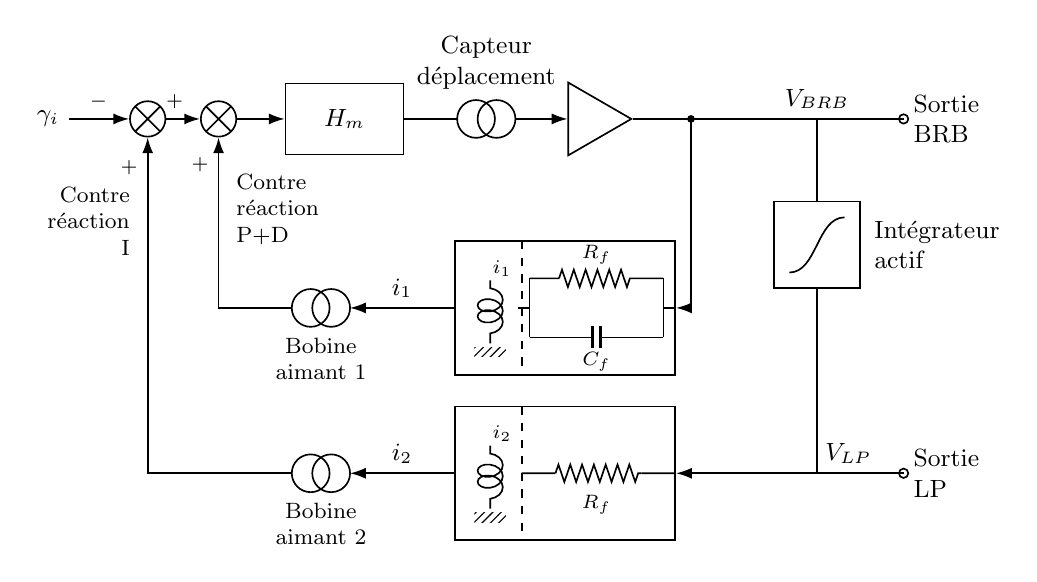
\begin{tikzpicture}[font=\small]
  \node[somme] (s1) at (0,0) {};
  \node[somme] (s2) at (0.9,0) {};
  \node[bloc] (h) at (2.5,0) {$H_m$};
  \pic (t) at (4.3,0) {transducteur}; \node[above=2.5mm, align=center] at (4.3,0) {Capteur\\déplacement};
  \node[gain] (a) at (5.6,0) {};
  \draw[->] (-1.0,0) node[left] {$\gamma_i$} -- (s1) node[above left, pos=0.8] {\scriptsize$-$};
  \draw[->] (s1) -- (s2) node[above left, pos=0.8] {\scriptsize$+$};
  \draw[->] (s2) -- (h); \draw (h) -- (t-o); \draw[->] (t-e) -- (a);
  \coordinate (nb) at (6.9,0); \fill (nb) circle (1.4pt);
  \draw (a.east) -- (9.6,0) node[circle, draw, inner sep=1.2pt] {} node[right, align=left] {Sortie\\BRB};
  \node[above] at (8.5,0) {$V_{BRB}$};
  % intégrateur
  \node[bloc, minimum width=1.1cm, minimum height=1.1cm] (int) at (8.5,-1.6) {};
  \draw (8.15,-1.95) .. controls (8.5,-1.95) and (8.5,-1.25) .. (8.85,-1.25);
  \node[right, align=left] at (9.1,-1.6) {Intégrateur\\actif};
  \draw (8.5,0) -- (int.north);
  \draw (int.south) -- (8.5,-4.5);
  \draw (6.9,-4.5) -- (9.6,-4.5) node[circle, draw, inner sep=1.2pt] {} node[right, align=left] {Sortie\\LP};
  \node[above] at (8.9,-4.5) {$V_{LP}$};
  % boucle P + D
  \boitier{(5.3,-2.4)}{pd}{1}{$i_1$}
  \pic (b1) at (2.2,-2.4) {transducteur};
  \node[below=2.5mm, align=center, font=\footnotesize] at (2.2,-2.4) {Bobine\\aimant 1};
  \draw[->] (nb) |- (pd.east);
  \draw[->] (pd.west) -- node[above] {$i_1$} (b1-e);
  \draw[->] (b1-o) -| (s2.south) node[below left, pos=0.97] {\scriptsize$+$};
  \node[align=left, font=\footnotesize, anchor=west] at (1.0,-1.15) {Contre\\réaction\\P+D};
  % boucle I
  \boitier{(5.3,-4.5)}{ii}{0}{$i_2$}
  \pic (b2) at (2.2,-4.5) {transducteur};
  \node[below=2.5mm, align=center, font=\footnotesize] at (2.2,-4.5) {Bobine\\aimant 2};
  \draw[->] (6.9,-4.5) -- (ii.east);
  \draw[->] (ii.west) -- node[above] {$i_2$} (b2-e);
  \draw[->] (b2-o) -| (s1.south) node[below left, pos=0.98] {\scriptsize$+$};
  \node[align=right, font=\footnotesize, left] at (-0.1,-1.3) {Contre\\réaction\\I};
\end{tikzpicture}
\end{document}
